
\documentclass[journal]{IEEEtran}
\usepackage[brazil]{babel}
\usepackage[utf8]{inputenc}
\usepackage[pdftex]{graphicx}

\begin{document}
	
%Titulo do artigo
\title{Controle e supervisão de um sistema de caldeira simulado}

%Nomes dos autores
\author{José Matheus Soares Ferreira 1~Jonatas Mendinça de Vasconcelos Brito 2~Thiago Marques Sousa 3~Daniel Alan Masquita de Vasconcelos~4% <-this % stops a space
\thanks{A. 1, Universidade Federal do Ceará, Sobral, Brasil, matrícula:412564}% <-this % stops a space
\thanks{A. 2, Universidade Federal do Ceará, Sobral, Brasil, matrícula:422569}% <-this % stops a space
\thanks{A. 3, Universidade Federal do Ceará, Sobral, Brasil, matrícula:412645}% <-this % stops a space
\thanks{A. 4, Universidade Federal do Ceará, Sobral, Brasil, matrícula:422104}
}

% The paper headers
\markboth{SBL0092 - SOFTWARE EM TEMPO REAL}%
{Shell \MakeLowercase{\textit{et al.}}: Bare Demo of IEEEtran.cls for IEEE Journals}


% make the title area
\maketitle

% As a general rule, do not put math, special symbols or citations
% in the abstract or keywords.
\begin{abstract}
Tanques são projetados para controlar e supervisionar processos industrias, afim de manter parâmetros com temperatura e nível controlados para a geração de um produto ou subproduto. Nesses casos, o controle deve ocorre em tempo real por meio da captação de sensores e pela ação de atuadores. Surgindo assim,  requisitos temporais que devem ser supridos por meio dos softwares em tempo real atrelados a sistemas computacionais capazes de compreender tais requisitos. Nele, o controle da temperatura no interior da caldeira deve se limitar a temperatura de referência definida pelo usuário e o controle de nível a altura pré estabelecida. Ambos os controles utilizam-se de parâmetros como fluxo de vasão de entrada, fluxo de vasão de saída, temperatura e altura, captados por sensores com periodicidade, atualidade, deadline e simultaneidade definidos.  
\end{abstract}

% Note that keywords are not normally used for peerreview papers.
\begin{IEEEkeywords}
Caldeira, controle de sistema, software em tempo real, mutex, sincronização e comunicação entre tarefas, seção crítica.
\end{IEEEkeywords}

\IEEEpeerreviewmaketitle

\section{Introdução}

\IEEEPARstart{s}{oftware} em tempo real, pode ser entendido como sistemas computacionais com requisitos de tempo real, sendo uma categoria especial de sistemas operacionais. Essa técnica, aplica-se a problemas que exijam requisitos com funcionalidades de natureza temporal não triviais, nesse sentido é essencial a confiabilidade no tempo de execução da tarefa e compatibilidade com prazos e requisitos definidos, ocasionando em resultados corretos logicamente e temporalmente\cite{IEEEhowto:romulo}.

Para os requisitos temporais, é necessário destacar que estão diretamente acoplados ao meio, no sentido de estarem fortemente associados com o mundo físico e que por isso a extração dos requisitos devem ocorrer na perspectiva do sistema responder ao estímulos do ambiente. Destacam-se os seguintes requisitos temporais:  periodicidade, Deadline, atualidade ou frescor dos dados e a simultaneidade dos dados\cite{IEEEhowto:romulo}.

Na aplicação de softwares de tempo real, a sincronização e a comunicação entre tarefas pode ocasionar inconsistência de dados e inversões de prioridades entre tarefas caso seja mal implementado. Para os trechos do código onde a tarefa acessa algum recurso compartilhado entre várias tarefas, é necessário definir uma seção crítica. Para evitar a inconsistência dos dados é usado o mecanismos do Mutex, "Técnica de sincronização que possibilita assegurar o acesso exclusivo (leitura e escrita) a um recurso compartilhado por duas ou mais entidades" \cite{IEEEhowto:Borges}, evitando que duas tarefas acessem ao mesmo tempo a memória. 

Nesse sentido, para acessar recursos compartilhados por outras tarefas é necessário definir mecanismos de sincronização para controlar o acesso de recursos e garantir que todos as tarefas possam executar suas seções críticas sem interferir com as seções críticas das outras tarefas.

Para programas concorrentes o problema da seção crítica é mais frequente, mas também existem  situações onde é necessário sincronizar tarefas que colaborem atráves de variáveis compartilhadas, nesses casos, usar apenas a exclusão mutua e Mutex pode gerar mais problemas. Portanto, é necessário definir outros padrões de sincronização como o semáforo e o monitor que são padrões para a programação concorrente com variáveis compartilhadas entre tarefas.

Dessa maneira, os monitores são módulos onde as interações entre tarefas acontecem. Para os monitores, a idéia é tornar determinados recursos privativo as tarefas \cite{IEEEhowto:romulo}. Nesse sentido, o monitor tenta quebrar o programa e recursos em módulos que são acessado as tarefas.. 

\section{Metodologia}

O método de sincronização e comunicação entre as tarefas propostas nesse trabalho é definido por meio do recurso de variáveis compartilhadas, portanto, definiu-se um sistema baseado em tarefas que realiza comunicação através de variáveis globais compartilhadas.

Nesse sentido, o trabalho basea-se em tarefas que são implementadas como thread de um mesmo processo, ou seja, o sistema é baseado em tarefas que são vistas pelo sistema operacional como thread.

Além disso,  é criado variáveis globais que são acessadas por várias tarefas (thread), permitindo diretamente a troca de dados. Dessa maneira, todas as threads automaticamente compartilham as variáveis globias do programa e as variáveis locais pertencentes a cada thread são tipicamente alocadas na  sua respectiva pilha, ou seja, são privadas. 

Afim de reduzir problemas tipicamente do método de sincronização e comunicação entre tarefas, como é o caso da inconsistência de dados, é garantindo que as threads acessem  variáveis compartilhadas executando sua seção crítica sem interferir com as seções críticas das outras threads. Para tanto, é utilizado o recurso do mutex, produzindo uma exclusão mútua, para evitar que várias tarefas acessem ao mesmo tempo uma variável. Bem como, o mecanismo de monitores que tenta quebrar os recursos em módulos, ao incapsular as variáveis globais, e a interação de acesso a esses recursos ocorre por meio da chamada de funções. 

%Apresente como o trabalho foi realizado, falando da Parte I e II da descrição. 

\subsection{Requisitos do Sistema}

Nesta primeira parte, os requisitos abaixo foram todos implementados e testados, logo em seguida.

\subsubsection{Requisito}Criação de uma thread periódica de 50ms para controlar a temperatura, onde a mesma foi criada no arquivo "controlemanual.c"; Inicialmente o algoritmo irá ler todas as variáveis globais e armazenar em variáveis locais e logo depois verificar a referência e calcular um valor proporcional para verificar a temperatura juntamente com um valor de erro, isso simultaneamente com o controle de nível.

\subsubsection{Requisito}Criação de uma thread, uma terafa periódica de 70ms para controlar o nível da água na caldeira. Essa tarefa é criada a partir de uma thread no arquivo "Esqueleto.c" chamada "thread\_controle\_nivel" onde, primeiramente é verificado se o nível da caldeira está alto ou baixo e logo em seguida verifica-se a temperatura, e com isso, ele irá atuar sobre o fluxo de água para cada caso;

\subsubsection{Requisito}Usar os atuadores Ni, Q, Na, Nf nas tarefas de controle. Assim, será possível controlar o nível pensando no controle da temperatura.

\subsubsection{Requisito}Criação da thread "thread\_le\_sensor" para mostrar os valores dos sensores Ta, T, Ti, No e H através dos monitores e do socket, além de atuar sobre os atuadores a cada 10 milissegundos."

\subsubsection{Requisito}Criação de uma thread de alarme para caso a temperatura ultrapasse 30 graus, onde a mesma foi criada na em "thread\_alarme";

\subsubsection{Requisito}Criação da thread "thread\_altera\_ref" para ler a entrada do teclado para alterar o valor de referência da temperatura e do nível determinado pelo usuário;

\subsubsection{Requisito}Criação da tarefa chamada "thread\_grava\_temp\_resp" para armazenar em arquivo os tempos de respostas da tarefa periódica do primeiro requisito em arquivo .txt nomeado de "dados\_tempo\_exec.txt", através de um buffer duplo (produtor/consumidor).

\subsubsection{Requisito}Criação de uma tarefa para armazenar e mostrar a cada 1 (um) segundo os valores dos sensores de nível (H) e de temperatura (T) em "thread\_mostra\_status" usando a função "aloca\_tela()" e "libera\_tela()" para mostrar os valores dos mesmos.

\subsection{Medições em Tempo Real}

Aqui, foram feitas as medições em tempo real da simulação em questão. Assim, podendo ser feitas análises, realizar experimentos e possíveis melhorias.

\subsubsection{Medição}

Obter o tempo mínimo e médio do tempo de resposta da tarefa periódica de controle de temperatura. Foi utilizado o programa de software Matlab para fazer a medição, o arquivo correspondente é “min\_max\_medio.m;

\subsubsection{Medição}

Obter o tempo de resposta máximo observado, também conhecido como Marca D’Água (HWM – High Water Mark). Diante dos dados apresentados, será possível afirmar os fatores importantes para saber se o deadline da tarefa de controle foi ou não suficiente e os fatores que contribuíram para que isso aconteça. Foi utilizado o programa de software Matlab para fazer a medição, o arquivo correspondente é “min\_max\_medio.m”;

\subsubsection{Medição}

Plotar um gráfico histograma e verificar a porcentagem de amostras que cumpririam o deadline definido;

\subsubsection{Medição}

Observar se a tarefa de controle de temperatura tem o Fator Skip 20. Plotar um gráfico mostrando apenas as medições onde o deadline foi perdido. Caso o sistema não possuir Fator Skip 20, explicar qual fator ele tem;

\subsubsection{Medição}

Observar se uma janela de 20 ativações consecutivas dos dados coletados das duas tarefas. Identificar o pior momento e com isso determinar qual valor de m para (m,20)-firme. Plotar um gráfico para cada tarefa mostrando o número de deadlines perdidos em uma janela de 20 ativações.

%Use diagrama de blocos se possível para indicar as etapas realizadas no trabalho.

\section{Resultados e discussões}

Apresente os resultados da parte I e II e discuta os resultados de acordo com o que foi pedido. Veja o exemplo de como colocar imagens no artigo. A Figura \ref{fig1} ...

	\begin{figure}[h]
	\centering
	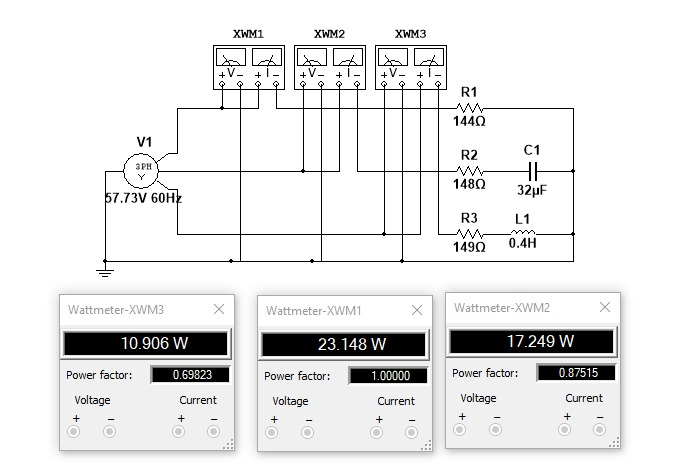
\includegraphics[width=3.5in]{Imagens/medidas.jpg}	
	\caption{Gráfico com as medições realizadas, na ordem dos casos de teste.}
	\label{fig1}
\end{figure}

%%%%%%%%%%%%%%%%%%%%%%%%%%%%%%%%%%%%%%%%%%%%%%%%5
%%%%%%%%%%%%%%%%%%%%%%%%%%%%%%%%%%%%%%%%%%%

\ifCLASSOPTIONcaptionsoff
  \newpage
\fi

\begin{thebibliography}{1}

\bibitem{IEEEhowto:romulo}
Oliveira, R. S. Fundamentos dos Sistemas de Tempo Real. Original registrado na Biblioteca Nacional. Primeira edição, revisão 3, outubro de 2018. ISBN-13: 9781728694047.

\bibitem{IEEEhowto:Borges}
Borges, V. B. Exclusão mútua (mutex). Departamento de Sistemas Eletrônicos Escola Politécnica da USP. 2017.

\end{thebibliography}

%%%%%%%%%%%%%%%%%%%%%%%%%%%%%%%%%%%%%%%%%
%Se tiver foto use essa forma
%%\begin{IEEEbiography}[{\includegraphics[width=1in,height=1.25in,clip,keepaspectratio]{Imagens/autor1.png}}]{Autor 1}
%%Texto da biografia aqui...
%%\end{IEEEbiography}




\end{document}
